\documentclass[11pt,letterpaper]{article}
\usepackage[lmargin=1in,rmargin=1in,bmargin=1in,tmargin=1in]{geometry}
\usepackage{checkins}

\pgfplotsset{soldot/.style={color=black,only marks,mark=*},
		holdot/.style={color=black,fill=white,only marks,mark=*},
		compat=1.12
}

% -------------------
% Content
% -------------------
\begin{document}
\thispagestyle{title}

% 08/22
\checkin{08/22} If $\ds\lim_{x \to 5} f(x)= -3$, then $f(5)= -3$. \pspace

\sol The statement is \textit{false}. A function's limit (if it even exists) \textit{does not} have to be the same as the function's value at that limiting value---the function does not even have to be defined there! Consider the three examples below. \par
	\begin{center}
	% Left
	\fbox{%
	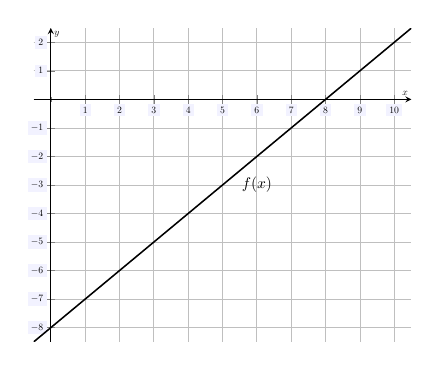
\begin{tikzpicture}[scale=0.7,every node/.style={scale=0.5}]
	\begin{axis}[
	grid=both,
	axis lines=middle,
	ticklabel style={fill=blue!5!white},
	xmin= -0.5, xmax=10.5,
	ymin= -8.5, ymax=2.5,
	xtick={-1,0,...,11},
	ytick={-8,-7,...,2},
	minor tick = {-9,-8,...,3},
	xlabel=\(x\),ylabel=\(y\),
	samples=20]
	\node at (6,-3) {\scalebox{1.6}{$f(x)$}};
	\addplot[thick, samples=5, domain= -0.5:10.5] {x - 8};
	\end{axis}
	\end{tikzpicture}
	} \hfill
	% Middle
	\fbox{%
	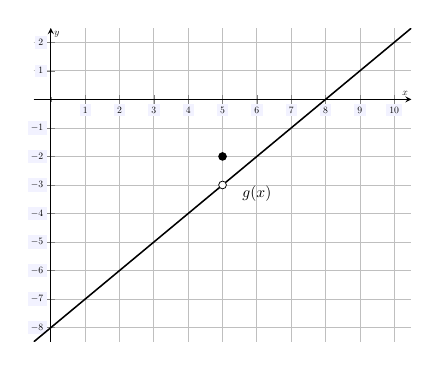
\begin{tikzpicture}[scale=0.7,every node/.style={scale=0.5}]
	\begin{axis}[
	grid=both,
	axis lines=middle,
	ticklabel style={fill=blue!5!white},
	xmin= -0.5, xmax=10.5,
	ymin= -8.5, ymax=2.5,
	xtick={-1,0,...,11},
	ytick={-8,-7,...,2},
	minor tick = {-9,-8,...,3},
	xlabel=\(x\),ylabel=\(y\),
	samples=20]
	\node at (6.0,-3.3) {\scalebox{1.6}{$g(x)$}};
	\addplot[thick, samples=5, domain= -0.5:10.5] {x - 8};
	\addplot[soldot] coordinates{(5,-2)};
	\addplot[holdot] coordinates{(5,-3)};
	\end{axis}
	\end{tikzpicture}
	} \hfill
	% Right
	\fbox{%
	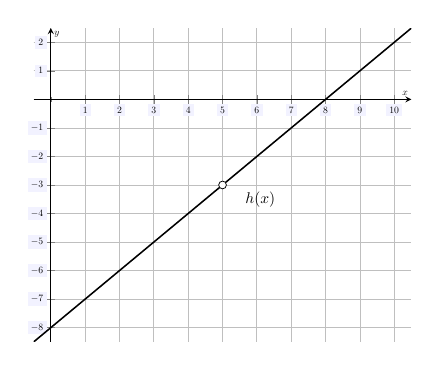
\begin{tikzpicture}[scale=0.7,every node/.style={scale=0.5}]
	\begin{axis}[
	grid=both,
	axis lines=middle,
	ticklabel style={fill=blue!5!white},
	xmin= -0.5, xmax=10.5,
	ymin= -8.5, ymax=2.5,
	xtick={-1,0,...,11},
	ytick={-8,-7,...,2},
	minor tick = {-9,-8,...,3},
	xlabel=\(x\),ylabel=\(y\),
	samples=20]
	\node at (6.1,-3.5) {\scalebox{1.6}{$h(x)$}};
	\addplot[thick, samples=5, domain= -0.5:10.5] {x - 8};
	\addplot[holdot] coordinates{(5,-3)};
	\end{axis}
	\end{tikzpicture}
	}
	\end{center} \par
For the graph of $f(x)$ on the left, $\ds\lim_{x \to 5} f(x)= -3$, so they are equal. However, observe that for $g(x)$ (the middle graph), we have $\ds\lim_{x \to 5} g(x)= -3$ but $g(5)= -2$, so that $\ds\lim_{x \to 5} g(x) \neq g(5)$. Similarly, in the graph of $h(x)$ on the right, $\ds\lim_{x \to 5} h(x)= -3$ but $h(-3)$ is not defined, so that $\ds\lim_{x \to 5} h(x) \neq h(-3)$. A function's value (if even defined) need not be related to its limit (if the limit even exists). \pvspace{1.3cm}



% 08/25
\checkin{08/25} The limit $\ds\lim_{x \to 0} \dfrac{\sin x}{x}= \text{DNE}$ because $\tfrac{\sin x}{x}$ becomes $\tfrac{0}{0}$ when one `plugs-in' $x= 0$ and $\frac{0}{0}$ is undefined. \pspace

\sol The statement is \textit{false}. In fact, $\ds\lim_{x \to 0} \dfrac{\sin x}{x}= 1$. Yes, $\tfrac{0}{0}$, $\pm\tfrac{\infty}{\infty}$, $0 \cdot \infty$, $\infty - \infty$, $0^0$, $1^\infty$, and $\infty^0$ are indeterminant/undefined expressions. However, that does not mean that the limit they arise from does not exist. The limit could exist or not---just like \textit{any} limit. `Running into' one of these expressions when evaluating a limit at its limiting value only means that one needs to try a different approach to determine if the limit exists or not. \pvspace{1.3cm}



% 08/27
\checkin{08/27} $\ds\lim_{x \to 0} \dfrac{\tan(5x)}{5x}= 1$ \pspace

\sol The statement is \textit{true}. Recall that $\ds\lim_{x \to 0} \dfrac{\sin(x)}{x}= 1$. We should think of this as $\ds\lim_{\Box \to 0} \dfrac{\sin \Box}{\Box}= 1$. But then\dots
	\[
	\lim_{x \to 0} \dfrac{\tan(5x)}{5x}= \lim_{x \to 0} \dfrac{\tfrac{\sin(5x)}{\cos(5x)}}{5x}= \lim_{x \to 0} \dfrac{\sin(5x)}{5x \cos x}= \lim_{x \to 0} \left( \dfrac{\sin(5x)}{5x} \cdot \dfrac{1}{\cos(5x)} \right)
	\]
Using the fact that $\ds\lim_{\Box \to 0} \dfrac{\sin \Box}{\Box}= 1$, we then have\dots
	\[
	\lim_{x \to 0} \dfrac{\tan(5x)}{5x}= \lim_{x \to 0} \left( \dfrac{\sin(5x)}{5x} \cdot \dfrac{1}{\cos(5x)} \right)= 1 \cdot \dfrac{1}{\cos(0)}= 1 \cdot \dfrac{1}{1}= 1
	\] \pvspace{1.3cm}



% 08/29
\checkin{08/29} $\ds\lim_{x \to 2^+} \dfrac{x - 3}{x - 2}= \infty$ \pspace

\sol The statement is \textit{false}. Observe that plugging-in $x= 2$, we obtain $\frac{-1}{0}$, which is undefined. However, this indicates that this is a `thinking limit'. Because in the limit, $x$ is `close' to 2, $x - 3$ is negative. As we approach 2 from the right, $x > 2$ so that $x - 2$ is positive. But then\dots
	\[
	\lim_{x \to 2^+} \dfrac{\overbrace{x - 3}^{-}}{\underbrace{x - 2}_{+}}= -\infty
	\] \pvspace{1.3cm}



% 09/03
\checkin{09/03} $\ds\lim_{x \to \infty} \dfrac{x^3 - 1}{1 - x^2}= -\infty$ \pspace

\sol The statement is \textit{true}. This is a rational limit. Observe that the degree of the numerator is 3 while the degree of the denominator is 2. Therefore, we know the limit will be $\pm\infty$. Observe that in the numerator, $x \to \infty$, so we know that $x^3 \to \infty$. In the denominator, we know that $x \to \infty$, so that $-x^2 \to -\infty$. Therefore, it should be that the limit tends to $-\infty$. We can confirm this intuition with the appropriate algebraic `trick': we divide the numerator and denominator by the `dominating' term in the denominator, which in this case is $x^2$:
	\[
	\lim_{x \to \infty} \dfrac{x^3 - 1}{1 - x^2}= \lim_{x \to \infty} \dfrac{x^3 - 1}{1 - x^2} \cdot \dfrac{1/x^2}{1/x^2}= \lim_{x \to \infty} \dfrac{\tfrac{x^3}{x^2} - \tfrac{1}{x^2}}{\tfrac{1}{x^2} - \tfrac{x^2}{x^2}}= \lim_{x \to \infty} \dfrac{x - \cancel{\tfrac{1}{x^2}}^{\,{}^0}}{\cancel{\tfrac{1}{x^2}}^{\,{}^0} - 1}= -\infty
	\] \pvspace{1.3cm}



% 09/05
\checkin{09/05} If $f(x)$ is a function and $\ds\lim_{x \to 1} f(x) = f(1)$, then $f(x)$ must be continuous at $x= 1$. \pspace

\sol The statement is \textit{true}. A function $f(x)$ is continuous at $x= a$ if $\ds f(a)= \lim_{x \to a} f(x)$. The statement of the problem states that $\ds\lim_{x \to 1} f(x)= f(1)$, i.e. $\ds f(1)= \lim_{x \to 1} f(x)$. Therefore, $f(x)$ is continuous at $x= 1$. Similarly, if we knew $f(x)$ was continuous at $x= 1$, then we would know that $\ds f(1)= \lim_{x \to 1} f(x)$. \pvspace{1.3cm}



% 09/07
\checkin{09/07} If $f(x)$ is given by\dots
	\[
	f(x)=
	\begin{cases}
	x + 1, & x \geq 0 \\
	4, & x < 0
	\end{cases}
	\]
Then $f(x)$ is differentiable at $x= 0$. \pspace

\sol The statement is \textit{false}. Recall that $f(x)$ is continuous at $x= a$ if $\ds f(a)= \lim_{x \to a} f(x)$ and that if a function is differentiable at $x= a$, then $f(x)$ is continuous at $x= a$. Therefore, $f(x)$ is continuous at $x= 0$ if and only if $\ds f(0)= \lim_{x \to 0} f(x)$. Observe that $f(0)= 0 + 1= 1$, $\ds\lim_{x \to 0^-} f(x)= \lim_{x \to 0^-} 4= 4$, and $\ds\lim_{x \to 0^+} f(x)= \lim_{x \to 0^+} (x + 1)= 0 + 1= 1$. Because $\ds\lim_{x \to 0^-} f(x) \neq \lim_{x \to 0^+} f(x)$, i.e. the left and right hand limits are not equal, $\ds\lim_{x \to 0} f(x)$ does not exist. But then $f(0) \neq \lim_{x \to 0} f(x)$, so that $f(x)$ is not continuous at $x= 0$. Because $f(x)$ is not continuous at $x= 0$, $f(x)$ cannot be differentiable at $x= 0$. \pspace

We can also verify this directly from the definition of the derivative. Recall that $\ds f'(a):= \lim_{h \to 0} \dfrac{f(a + h) - f(a)}{h}$. Here, we have $a= 0$ and $f(0)= 0 + 1= 1$. We compute this limit by computing the left and right hand limits. We have\dots
	\[
	\begin{aligned}
	\lim_{h \to 0^-} \dfrac{f(0 + h) - f(0)}{h}= \lim_{h \to 0^-} \dfrac{f(h) - f(0)}{h}= \lim_{h \to 0^-} \dfrac{4 - 1}{h}= \lim_{h \to 0^-} \dfrac{3}{h}= -\infty \\[0.3cm]
	\lim_{h \to 0^+} \dfrac{f(0 + h) - f(0)}{h}= \lim_{h \to 0^+} \dfrac{f(h) - f(0)}{h}= \lim_{h \to 0^+} \dfrac{(h + 1) - 1}{h}= \lim_{h \to 0^+} 1= 1 \\
	\end{aligned}
	\]
Because $\ds \lim_{h \to 0} \dfrac{f(0 + h) - f(0)}{h}$ does not exist, $f'(0)$ does not exist, i.e. $f(x)$ is not differentiable at $x= 0$. \pvspace{1.3cm}



% 09/10
\checkin{09/10} $\dfrac{d}{dx} \left( e^{\sin x} \right)= e^{\cos x}$ \pspace

\sol The statement is \textit{false}. Observe that the given solution, $e^{\cos x}$, has the derivative of both $e^x$ (which is $e^x$) and $\sin x$ (which is $\cos x$) simultaneously. However, all the derivative rules only ever have one taking the derivative of \textit{one} function at a time for any corresponding term. If we choose $f(x)= e^x$ and $g(x)= \sin x$, we have $f \big( g(x) \big)= f(\sin x)= e^{\sin x}$. We know that $f'(x)= e^x$ and $g'(x)= \cos x$. Using the chain rule, $\tfrac{d}{dx} f \big( g(x) \big)= f' \big( g(x) \big) \cdot g'(x)$, we have $\tfrac{d}{dx} e^{\sin x}= e^{\sin x} \cdot \cos x= e^{\sin x} \cos x$. Alternatively, using the `box method' or `onion approach', the first `layer' is $e^\Box{}$, whose derivative is $e^\Box{}$. We multiply by the derivative of the contents of $\Box{}$, which is the derivative of $\sin x$, i.e. $\cos x$. But then the derivative is $e^{\sin x} \cos x$. \pvspace{1.3cm}



% 09/11
\checkin{09/11} $\dfrac{d}{dx} \,\left( x^4 \csc(x) e^x \right)= 4x^3 \cdot \csc(x) e^x + -\csc x \cot x \cdot x^4 e^x + e^x \cdot x^4 \csc x$ \pspace

\sol The statement is \textit{true}. Although we can use the Product Rule: $\dfrac{d}{dx} (fg)= f'g + fg'$, it is simpler to recall that the Product Rule is a `one at a time rule.' That is, the product rule says to add together the product of the terms where the derivative of only one of the terms has been taken. Using this approach, we have\dots
	\[
	\begin{aligned}
	\dfrac{d}{dx} \,\left( x^4 \csc(x) e^x \right)&= \dfrac{d}{dx} (x^4) \cdot \csc x e^x + \dfrac{d}{dx} (\csc x) \cdot x^4 e^x + \dfrac{d}{dx}(e^x) \cdot x^4 \csc x \\[0.3cm]
	&= 4x^3 \cdot \csc(x) e^x + -\csc x \cot x \cdot x^4 e^x + e^x \cdot x^4 \csc x
	\end{aligned}
	\] \pvspace{1.3cm}



% 09/15
\checkin{09/15} $\dfrac{d}{dx} \left( \dfrac{x^2}{4x - 3} \right)= \dfrac{4(x^2) - 2x(4x - 3)}{(4x - 3)^2}$ \pspace

\sol The statement is \textit{false}. Recall that the quotient rule is given by $\frac{d}{dx} \left( \frac{f}{g} \right)= \frac{f' g - g' f}{g^2}$, i.e. the derivative of the bottom `gets the negative for its derivative' or the `\textbf{\underline{n}}umerator function' gets the \textbf{\underline{n}}egative. Observe that the given solution has the order of subtraction in the numerator reversed, i.e. it is the negative of the correct answer; that is, the numerator is `backwards' from the actual quotient rule. The correct answer should be:
	\[
	\dfrac{d}{dx} \left( \dfrac{x^2}{4x - 3} \right)= \dfrac{2x(4x - 3) - 4(x^2)}{(4x - 3)^2}
	\] \pvspace{1.3cm}



% 09/17
\checkin{09/17} If $f(x)$ is a function with $f(1)= 3$ and $f'(1)= 10$, then it should be that $f(0.8) \approx 1$. \pspace

\sol The statement is \textit{true}. The linearization of $f(x)$ at $x= a$ is $\ell_a(x)= f(a) + f'(a) \,\big( x - a \big)$. We know that if $x$ is `close' to $a$, then $f(x) \approx \ell_a(x)$. The linearization of the given $f(x)$ at $x= 1$ is $\ell_1(x)= f(1) + f'(1) \,\big( x - 1 \big)= 3 + 10(x - 1)$. But then we have\dots
	\[
	f(0.8) \approx \ell_1(0.8)= 3 + 10(0.8 - 1)= 3 + 10(-0.2)= 3 + (-2)= 1
	\] \pvspace{1.3cm}



% 09/24
\checkin{09/24} The critical value(s) for $f(x)= 2x + \frac{1}{x^2}$ is $x= 1$. \pspace

\sol The statement is \textit{false}. Recall the critical value(s) for a function $f(x)$ are the value(s) for which $f'(x)$ is 0 or undefined. Because $f(x)= 2x + \frac{1}{x^2}= 2x + x^{-2}$, we have $f'(x)= 2 - 2x^{-3}= 2 - \frac{2}{x^3}$. Observe that $f'(x)$ is undefined at $x= 0$, so that $x= 0$ is a critical value. Solving $f'(x)= 0$, we have\dots
	\[
	\begin{gathered}
	f'(x)= 0 \\
	2 - \frac{2}{x^3}= 0 \\
	2= \frac{2}{x^3} \\
	2x^3= 2 \\
	x^3= 1 \\
	x= 1
	\end{gathered}
	\]
Therefore, $x= 1$ is a critical value. Therefore, the critical values are $x= 0, 1$. \pvspace{1.3cm}



% 09/26
\checkin{09/26} $\ds\lim_{x \to 0} \dfrac{\sin(4x)}{5x} \stackrel{\text{LH}}{=} \lim_{x \to 0} \dfrac{4\cos(4x)}{5}= \dfrac{4}{5}$ \pspace

\sol The statement is \textit{true}. Na\"ively evaluating the argument at $x= 0$, we obtain $\frac{0}{0}$. But then l'H\^{o}pital's should apply. The derivative of $\sin(4x)$ is $\cos(4x) \cdot 4= 4 \cos(4x)$ and the derivative of $5x$ is $5$. But then\dots
	\[
	\lim_{x \to 0} \dfrac{\sin(4x)}{5x} \stackrel{\text{LH}}{=} \lim_{x \to 0} \dfrac{4\cos(4x)}{5}= \dfrac{4 \cos(0)}{5}= \dfrac{4(1)}{5}= \dfrac{4}{5}
	\]
However, we can also recognize this as a `special limit', $\ds\lim_{\Box{} \to 0} \dfrac{\sin \Box{}}{\Box{}}= 1$, and solve it this way:
	\[
	\lim_{x \to 0} \dfrac{\sin(4x)}{5x}= \lim_{x \to 0} \dfrac{1}{5} \dfrac{\sin(4x)}{x}= \lim_{x \to 0} \dfrac{1}{5} \dfrac{\sin(4x)}{4x} \cdot 4= \dfrac{1}{5} \cdot 1 \cdot 4= \dfrac{4}{5}
	\] \pvspace{1.3cm}



% 09/29
\checkin{09/29} $\ds\lim_{x \to 1} \dfrac{3x^2 - 2x - 1}{x^2 - 2x + 1} \stackrel{\text{L.H.}}{=} \lim_{x \to 1} \dfrac{6x - 2}{2x - 2} \stackrel{\text{L.H.}}{=} \dfrac{6}{2}= 3$ \pspace

\sol The statement is \textit{false}. Na\"ively plugging in $x= 1$ into $\dfrac{3x^2 - 2x - 1}{x^2 - 2x + 1}$, we obtain $\frac{0}{0}$, so l'H\^{o}pital's rule applies. Applying l'H\^{o}pital's rule, we obtain $\ds\lim_{x \to 1} \dfrac{6x - 2}{2x - 2}$. However, now na\"ively plugging in $x= 1$, we obtain $\frac{4}{0}$ and l'H\^{o}pital's rule does not apply. Indeed, this is now a `thinking limit.' One can show that this limit does not exist. [In fact, this shows the initial application does not necessarily hold. However, $\dfrac{3x^2 - 2x - 1}{x^2 - 2x + 1}= \dfrac{(3x + 1)(x - 1)}{(x - 1)^2}$. But then $\ds\lim_{x \to 1} \dfrac{3x^2 - 2x - 1}{x^2 - 2x + 1}= \lim_{x \to 1} \dfrac{3x + 1}{x - 1}$ and this limit does not exist.] \pvspace{1.3cm}



% 10/01
\checkin{10/01} $\ds\lim_{x \to 0^+} \left( \dfrac{1}{\sin x} - \dfrac{1}{x} \right) \stackrel{\text{L.H.}}{=} \lim_{x \to 0^+} \left( \dfrac{1}{\cos x} - \dfrac{1}{1} \right)$ \pspace

\sol The statement is \textit{false}. Observe that if one na\"ively evaluates $\dfrac{1}{\sin x} - \dfrac{1}{x}$ at $x= 0$, one obtains $\infty - \infty$, which is indeterminant. However, we recognize this as a limit to which l'H\^opital's will typically be applied to. However, l'H\^opital's rule does not immediately apply as it can only be used in the case of the indeterminant forms $\frac{0}{0}$ or $\pm \frac{\infty}{\infty}$. Even if l'H\^opital's rule could be applied, recall that it says that if $\ds\lim \frac{f}{g}$ is $\frac{0}{0}$ or $\pm \frac{\infty}{\infty}$, then $\ds\lim \frac{f}{g}= \lim \frac{f'}{g'}$ (so long as $\ds\lim \frac{f'}{g'}$ exists). So, even if l'H\^opital's rule applied, it would have not been applied correctly here because there was not a single fraction and `l'H\^opital's was applied' to only the denominators of the separate fractions. \pspace

In the case of the indeterminant form $\infty - \infty$, we often factor a term out or combine terms. In this case, creating a common denominator, we have\dots
	\[
	\lim_{x \to 0^+} \left( \dfrac{1}{\sin x} - \dfrac{1}{x} \right)= \lim_{x \to 0^+} \dfrac{x - \sin x}{x \sin x}
	\]
Observe that now na\"ively evaluating $\dfrac{x - \sin x}{x \sin x}$ at $x= 0$, one obtains $\frac{0}{0}$. But then l'H\^opital's rule applies. So, we have\dots
	\[
	\lim_{x \to 0^+} \dfrac{x - \sin x}{x \sin x} \stackrel{\text{L.H.}}{=} \lim_{x \to 0^+} \dfrac{1 - \cos x}{\sin x + x \cos x}
	\]
Na\"ively evaluating $\dfrac{1 - \cos x}{\sin x + x \cos x}$ at $x= 0$, we obtain $\frac{0}{0}$. So, we use l'H\^opital's again: 
	\[
	\lim_{x \to 0^+} \dfrac{1 - \cos x}{\sin x + x \cos x} \stackrel{\text{L.H.}}{=} \lim_{x \to 0^+} \dfrac{\sin x}{\cos x + (\cos x - x \sin x)}= \lim_{x \to 0^+} \dfrac{\sin x}{2 \cos x - x \sin x}= \dfrac{0}{2(1) - 0}= 0
	\]
Therefore, $\\lim_{x \to 0^+} \left( \dfrac{1}{\sin x} - \dfrac{1}{x} \right)= 0$. \pvspace{1.3cm}



% 10/03
\checkin{10/03} $\dfrac{d}{dt} \left( x \sin(xy) \right)= x' \sin(xy) + x \cos(xy) \big(x' y + y' x)$ \pspace

\sol The statement is \textit{true}. If $x, y$ do not depend on $t$, then clearly $\dfrac{d}{dt} \left( x \sin(xy) \right)= 0$. However, if we do not know this to be the case, we can always implicitly differentiate, which will give us a correct answer regardless of whether $x, y$ depends on $t$. Assuming $x, y$ might depend on $t$, observe that $x \sin(xy)$ is a product of functions which depend on $t$. So, we need a product rule (which will also require a chain rule for the term $\sin(xy)$):
	\[
	\begin{aligned}
	\dfrac{d}{dt} \left( x \sin(xy) \right)&= \dfrac{d}{dt}(x) \cdot \sin(xy) + x \cdot \dfrac{d}{dt} \big( \sin(xy) \big) \\
	&= \frac{dx}{dt}\, \sin(xy) + x \cos(xy) \cdot \dfrac{d}{dt} (xy) \\
	&= \frac{dx}{dt}\, \sin(xy) + x \cos(xy) \cdot \left( \dfrac{d}{dt}(x) \cdot y + x \cdot \dfrac{d}{dt}(y) \right) \\
	&= \frac{dx}{dt}\, \sin(xy) + x \cos(xy) \cdot \left( \dfrac{dx}{dt}(x) \cdot y + x \cdot \dfrac{dy}{dt} \right) \\
	&= x' \sin(xy) + x \cos(xy) \,(x' y+ y' x)
	\end{aligned}
	\] \pvspace{1.3cm}



% 10/06
\checkin{10/06} One can substitute anything that is constant throughout the problem into the equation to be differentiated in a related rates problem without introducing an error. \pspace

\sol The statement is \textit{true}. This is easiest seen in an example. Suppose we had a problem where the side lengths of a right triangle were changing in time but one side was constant. Say that $a, b$ and $c$ were the legs and hypotenuse of the triangle, respectively, and that $a, c$ were changing in time but $b$ was not. We know that $a^2 + b^2= c^2$. Because $b$ is constant with respect to time, we could substitute it before differentiating with respect to time. Say that $b= 5$. We would then have\dots
	\[
	\begin{gathered}
	a^2 + b^2= c^2 \\
	a^2 + 5^2= c^2 \\
	\dfrac{d}{dt} \,(a^2 + 5^2)= \dfrac{d}{dt} \,c^2 \\
	2aa' + 0= 2cc' \\
	2aa'= 2cc' \\
	aa'= cc'
	\end{gathered}
	\]
We did not \textit{have} to substitute this $b$-value. If we had not, we would have\dots
	\[
	\begin{gathered}
	a^2 + b^2= c^2 \\
	\dfrac{d}{dt} \,(a^2 + b^2)= \dfrac{d}{dt} \,c^2 \\
	2aa' + 2bb'= 2cc' \\
	aa' + bb'= cc'
	\end{gathered}
	\]
Why is the same as the original answer above? If $b$ is constant with respect to time, then $b'= 0$ because $b$ is not changing. But then\dots
	\[
	\begin{gathered}
	aa' + bb'= cc' \\
	aa' + b(0)= cc' \\
	aa'= cc' 
	\end{gathered}
	\]
However, suppose that $b$ was \textit{not} constant with respect to time but we still had $b= 5$ at some moment in time. If we substituted it as above, we would obtain the same result as we did in the original answer, $aa'= cc'$, where we should have obtained $aa' + bb'= cc'$ as we did in the second answer. So, in a related rates problem, one can only substitute values which are constant with respect to the differentiated variable before differentiating. \pvspace{1.3cm}



% 010/08
\checkin{10/08} $\dfrac{d}{dx}\,(y^2 \cdot y')= 2y \cdot y' + y^2 \cdot y''$ \pspace

\sol The statement is \textit{false}. The answer given in the problem statement has missed the $y'$ term produced by differentiating $y^2$ implicitly---likely because of the $y'$ term already present. We have\dots
	\[
	\dfrac{d}{dx}\,(y^2 \cdot y')= \dfrac{d}{dx}(y^2) \cdot y' + y^2 \cdot \dfrac{d}{dx}(y')= (2yy') \cdot y' + y^2 \cdot y''= 2y (y')^2 + y^2 \cdot y''
	\] \pvspace{1.3cm}



% 010/13
\checkin{10/13} It is often easier to work with the square of the distance between two points rather than the distance itself, and this approach will often yield the same answer in the end. \pspace

\sol The statement is \textit{true}. Although this is not necessarily universally true, this is often the case. Consider the example when we want to determine how the distance from a point $(x, y)$ to the point $(1, -2)$ changes in time. The distance is $d= \sqrt{(x - 1)^2 + \big(y - (-2) \big)^2}= \sqrt{(x - 1)^2 + (y + 2)^2}$. Then the rate of change of this distance in time is\dots
	\[
	d'= \dfrac{d}{dt}\, \sqrt{(x - 1)^2 + \big(y - (-2) \big)^2}= \dfrac{2(x - 1) x' + 2(y + 2) y'}{2 \sqrt{(x - 1)^2 + \big(y + 2 \big)^2}}= \dfrac{(x - 1) x' + (y + 2) y'}{\sqrt{(x - 1)^2 + \big(y + 2 \big)^2}}
	\]
Although this derivative is not necessarily that difficult, it is tedious. Compare to this to workin with $d^2= (x - 1)^2 + (y + 2)^2$. Differentiating in time, we have\dots
	\[
	\begin{gathered}
	\dfrac{d}{dt}\, d^2= \dfrac{d}{dt}\, \left[ (x - 1)^2 + (y + 2)^2 \right] \\
	2dd'= 2(x - 1) x' + 2(y + 2) y' \\
	dd'= (x - 1) x' + (y + 2) y'
	\end{gathered}
	\]
This is just as easy to find $d'$ for---perhaps easier---given $x, y, x', y'$ than the expression we found before. We can even find the same equation as above. We know that $d= \sqrt{(x - 1)^2 + (y + 2)^2}$. But then\dots
	\[
	\begin{gathered}
	dd'= (x - 1) x' + (y + 2) y' \\
	d'= \dfrac{(x - 1) x' + (y + 2) y'}{d} \\
	d'= \dfrac{(x - 1) x' + (y + 2) y'}{\sqrt{(x - 1)^2 + (y + 2)^2}}
	\end{gathered}
	\]
This same strategy will also be useful for optimization as well. \pvspace{1.3cm}



% 010/15
\checkin{10/15} If $x_0$ is a local minimum for $d^2= (x - 1)^2 + \big( f(x) + 4 \big)^2$, then it is a minimum for $d= \sqrt{(x - 1)^2 + \big( f(x) + 4 \big)^2}$. \pspace

\sol The statement is \textit{true}. The distance between a point on a function, $f(x)$, i.e. $\big(x, f(x) \big)$, and a point $(1, -4)$ is given by\dots
	\[
	d= \sqrt{(x_1 - x_2)^2 + (y_1 - y_2)^2}= \sqrt{(x - 1)^2 + \big(f(x) - (-4) \big)^2}= \sqrt{(x - 1)^2 + \big(f(x) + 4 \big)^2}
	\]
While minimizing/maximizing $d^2$ instead of $d$ may result in different minimum/maximum \textit{values}, the location of these minimum/maximum values remains the same. That is, $d^2$ and $d$ have the same critical values. So, instead of minimizing/maximizing $d$, we can minimize/maximize $d^2$, which is simpler to work with because of the lack of square root, c.f. the previous check-in. \pvspace{1.3cm}



























\end{document}